Let us for a moment consider a single quadrilateral element in the $xy$-plane, 
as shown on the following figure:
\begin{center}
\includegraphics[width=5.8cm]{images/shape.png}
\end{center}
Let us assume that we know the values of a given field $u$ at the vertices.
For a given point $M$ inside the element in the plane, what is the value of the 
field $u$ at this point?
It makes sense to postulate that $u_M=u(x_M,y_M)$ will be given  by 
\[
u_M= \phi(u_1,u_2,u_3,u_4,x_M,y_M) 
\]
where $\phi$ is a function to be determined. Although $\phi$ is not unique, we can 
decide to express the value $u_M$ as a weighed sum of the values at the vertices $u_i$.
One option could be to assign all four vertices the same weight, say $1/4$ so that 
$u_M=(u_1+u_2+u_3+u_4)/4$, i.e. $u_M$ is simply given by the arithmetic mean 
of the vertices values. This approach suffers from a major drawback as it does
not use the location of point $M$ inside the element. For instance, when 
$(x_M,y_M) \rightarrow (x_2,y_2)$ we expect $u_M \rightarrow u_2$.

In light of this, we could now assume that the weights would depend on the position 
of $M$ in a continuous fashion:
\[
u(x_M,y_M) = \sum_{i=1}^4 N_i(x_M,y_M)\;  u_i
\]
where the $N_i$ are continous ("well behaved") functions which have the property:
\[
N_i(x_j,y_j)=\delta_{ij}
\]
or, in other words: 
\begin{eqnarray}
N_3(x_1,y_1) &=& 0 \\
N_3(x_2,y_2) &=& 0 \\
N_3(x_3,y_3) &=& 1 \\
N_3(x_4,y_4) &=& 0 
\end{eqnarray}
The functions $N_i$ are commonly called basis functions. \index{basis functions}

Omitting the $M$ subscripts for any point inside the element, the velocity components $u$
and $v$ are given by:
\begin{eqnarray}
\hat{u}(x,y) &=& \sum_{i=1}^4 N_i(x,y)\;  u_i \\
\hat{v}(x,y) &=& \sum_{i=1}^4 N_i(x,y)\;  v_i \label{bf01}
\end{eqnarray}
Rather interestingly, one can now easily compute velocity gradients (and therefore the 
strain rate tensor) since we have assumed the basis functions to be "well behaved" 
(in this case differentiable):
\begin{eqnarray}
\dot{\epsilon}_{xx}(x,y) &=& \frac{\partial u}{\partial x} = \sum_{i=1}^4 \frac{\partial N_i}{\partial x}\;  u_i \\
\dot{\epsilon}_{yy}(x,y) &=& \frac{\partial v}{\partial y} = \sum_{i=1}^4 \frac{\partial N_i}{\partial y}\;  v_i \\
\dot{\epsilon}_{xy}(x,y) &=& \frac{1}{2}\frac{\partial u}{\partial y} 
+ \frac{1}{2}\frac{\partial v}{\partial x} 
= \frac{1}{2}\sum_{i=1}^4 \frac{\partial N_i}{\partial y}\;  u_i
+ \frac{1}{2}\sum_{i=1}^4 \frac{\partial N_i}{\partial x}\;  v_i
\end{eqnarray}
How we actually obtain the exact form of the basis functions is explained in the coming section.













%%%%%%%%%%%%%%%%%%%%%%%%%%%%%%%%%%%%
\subsubsection{The $Q_1$ basis in 2D}

In this section, we place ourselves in the most favorables case, i.e. the element is a square defined 
by $-1<r<1$, $-1<s<1$ in the Cartesian coordinates system $(r,s)$:

\begin{center}
\includegraphics[height=5cm]{images/element_rs.png}\\
{\color{red} add corner numbering}
\end{center}

This element is commonly called the reference element. How we go from the $(x,y)$ coordinate system 
to the $(r,s)$ once and vice versa will be dealt later on.
For now, the basis functions in the above reference element and in the reduced 
coordinates system $(r,s)$ are given by:

\begin{eqnarray}
N_1(r,s)&=&0.25(1-r)(1-s) \nonumber\\
N_2(r,s)&=&0.25(1+r)(1-s) \nonumber\\
N_3(r,s)&=&0.25(1+r)(1+s) \nonumber\\
N_4(r,s)&=&0.25(1-r)(1+s) \nonumber
\end{eqnarray}

The partial derivatives of these functions with respect to $r$ ans $s$ automatically follow:

\begin{eqnarray}
\frac{\partial N_1}{\partial r}(r,s)&=& - 0.25(1-s) \nonumber\\
\frac{\partial N_2}{\partial r}(r,s)&=& + 0.25(1-s) \nonumber\\
\frac{\partial N_3}{\partial r}(r,s)&=& + 0.25(1+s) \nonumber\\
\frac{\partial N_4}{\partial r}(r,s)&=& - 0.25(1+s) \nonumber
\end{eqnarray}

\begin{eqnarray}
\frac{\partial N_1}{\partial s}(r,s)&=& - 0.25(1-r) \nonumber\\
\frac{\partial N_2}{\partial s}(r,s)&=& - 0.25(1+r) \nonumber\\
\frac{\partial N_3}{\partial s}(r,s)&=& + 0.25(1+r) \nonumber\\
\frac{\partial N_4}{\partial s}(r,s)&=& + 0.25(1-r) \nonumber
\end{eqnarray}

Let us go back to Eq.(\ref{bf01}). And let us assume that the function $v(r,s)=C$ so that $v_i=C$ for $i=1,2,3,4$. 
It then follows that 
\[
\hat{v}(r,s) = \sum_{i=1}^4 N_i(r,s)\;  v_i = C \sum_{i=1}^4 N_i(r,s)
=C [
N_1(r,s)
+N_2(r,s)
+N_3(r,s)
+N_4(r,s)]=C
\]
This is a very important property: if the $v$ function used to assign values at the vertices is constant, then 
the value of $\hat{v}$ {\it anywhere} in the element is exactly $C$.
If we now turn to the derivatives of $v$ with respect to $r$ and $s$:
\[
\frac{\partial \hat{v}}{\partial r}(r,s) = \sum_{i=1}^4 \frac{\partial N_i}{\partial r}(r,s)\;  v_i = C \sum_{i=1}^4 \frac{\partial N_i}{\partial r}(r,s) 
= C \left[ - 0.25(1-s)  + 0.25(1-s)  + 0.25(1+s)  - 0.25(1+s) \right] = 0 
\]

\[
\frac{\partial \hat{v}}{\partial s}(r,s) = \sum_{i=1}^4 \frac{\partial N_i}{\partial s}(r,s)\;  v_i = C \sum_{i=1}^4 \frac{\partial N_i}{\partial s}(r,s) 
= C \left[ - 0.25(1-r) - 0.25(1+r) + 0.25(1+r) + 0.25(1-r) \right] = 0 
\]
We reassuringly find that the derivative of a constant field anywhere in the element is exactly zero.

If we now choose $v(r,s)=ar+bs$ with $a$ and $b$ two constant scalars, we find:
\begin{eqnarray}
\hat{v}(r,s) 
&=& \sum_{i=1}^4 N_i(r,s)\;  v_i  \\
&=& \sum_{i=1}^4 N_i(r,s) (ar_i+bs_i) \\
&=& a \underbrace{\sum_{i=1}^4 N_i(r,s) r_i}_{r} + b \underbrace{\sum_{i=1}^4 N_i(r,s) s_i}_{s} \\
&=& a \left[ 
0.25(1-r)(1-s)(-1)
+0.25(1+r)(1-s)(+1)
+0.25(1+r)(1+s)(+1)
+0.25(1-r)(1+s)(-1) \right]  \nonumber\\
&+& b  
\left[ 
0.25(1-r)(1-s)(-1)
+0.25(1+r)(1-s)(-1)
+0.25(1+r)(1+s)(+1)
+0.25(1-r)(1+s)(+1) \right]  \nonumber\\
&=& a \left[ 
-0.25(1-r)(1-s)
+0.25(1+r)(1-s)
+0.25(1+r)(1+s)
-0.25(1-r)(1+s) \right]  \nonumber\\
&+& b  
\left[ 
-0.25(1-r)(1-s)
-0.25(1+r)(1-s)
+0.25(1+r)(1+s)
+0.25(1-r)(1+s) \right]  \nonumber\\
&=& ar+bs
\end{eqnarray}
{\color{red} verify above eq}.
This set of bilinear shape functions is therefore capable of exactly representing a bilinear field.
The derivatives are:
\begin{eqnarray}
\frac{\partial \hat{v}}{\partial r}(r,s) 
&=& \sum_{i=1}^4 \frac{\partial N_i}{\partial r}(r,s)\;  v_i  \\
&=& a \sum_{i=1}^4 \frac{\partial N_i}{\partial r}(r,s) r_i + b \sum_{i=1}^4 \frac{\partial N_i}{\partial r}(r,s) s_i \\
&=& a \left[
- 0.25(1-s)(-1) 
+ 0.25(1-s)(+1) 
+ 0.25(1+s)(+1) 
- 0.25(1+s)(-1) 
\right] \nonumber\\
&+&b \left[
- 0.25(1-s)(-1) 
+ 0.25(1-s)(-1) 
+ 0.25(1+s)(+1) 
- 0.25(1+s)(+1) 
\right] \nonumber\\
&=& \frac{a}{4} \left[
 (1-s)
+ (1-s)
+ (1+s)
+ (1+s)
\right] \nonumber\\
&+&\frac{b}{4} \left[
 (1-s)
- (1-s)
+ (1+s)
- (1+s)
\right] \nonumber\\
&=& a 
\end{eqnarray}
Here again, we find that the derivative of the bilinear field inside the element is exact: 
$\frac{\partial \hat{v}}{\partial r} = \frac{\partial v}{\partial r}$.

However, following the same methodology as above, one can easily prove that this is no more true for polynomials of degree strivtly higher than 1. This fact has serious consequences: if the solution to the problem at hand is for instance a parabola, the $Q_1$ shape functions cannot represent the solution properly, but only by approximating the parabola in each element by a line. As we will see later, $Q_2$ basis functions can remedy this problem by containing themselves quadratic terms.

%%%%%%%%%%%%%%%%%%%%%%%%%%%%%%%%%%%%
\subsubsection{The $Q_2$ basis in 2D}




